% !TEX root = ../../main.tex
\section{Sơ đồ nguyên lý và kết nối hệ thống điện}
\label{sec:design-electrical-system}
% Block PNGs copied from hardware/kicad at commit 4952fd9 (update-hardware).

\begin{figure}[H]
	\centering
	% Functional connections summarized from the three electrical block schematics.
\begin{tikzpicture}[
		x=1cm,y=1cm,>=latex,line width=0.8pt,
		font=\fontsize{11}{13}\selectfont,
		block/.style={draw,fill=gray!6,align=center,inner sep=6pt,
				minimum height=1.45cm},
		every node/.style={align=center}
	]
	\node[block,text width=5.0cm] (power) at (6.25,2.7)
	{\textbf{Khối nguồn}\\Pin LiPo 3S};
	\node[block,text width=4.8cm] (control) at (2.6,0)
	{\textbf{Khối điều khiển}\\STM32F103VET6\\BMI160, BNO055, bộ thu ELRS};
	\node[block,text width=4.6cm] (actuators) at (10.0,0)
	{\textbf{Khối cơ cấu chấp hành}\\Bốn ESC, động cơ\\và cánh quạt};

	\draw[->] (power.east) -| node[pos=0.7,right] {Nguồn pin 3S} (actuators.north);
	\draw[->,dashed] (control.east) -- node[above] {PWM} (actuators.west);
	\draw[->] (actuators.south) -- ++(0,-0.65)
	-| node[pos=0.25,below] {5 V từ BEC của ESC2} (control.south);
	\node[font=\fontsize{10}{12}\selectfont] at (6.25,-2.6)
	{Đường liền: cấp nguồn; đường nét đứt: tín hiệu điều khiển.\\Ba khối dùng chung GND.};
\end{tikzpicture}

	\caption{Sơ đồ khối chức năng của hệ thống điện quadrotor.}
	\label{fig:design-electrical-blocks}
\end{figure}

Hệ thống điện trong \fref{fig:design-electrical-blocks} gồm ba khối chức năng: khối nguồn, khối điều khiển và khối cơ cấu chấp hành. Pin LiPo 3S cấp nguồn cho bốn ESC, còn STM32 gửi lệnh PWM đến từng ESC để điều khiển động cơ. Nhánh BEC của ESC2 cấp nguồn 5 V cho khối điều khiển; các khối dùng chung GND.

\subsection{Mạch cấp nguồn và phân phối điện áp}
\label{subsec:design-power-block}

\begin{figure}[H]
	\centering
	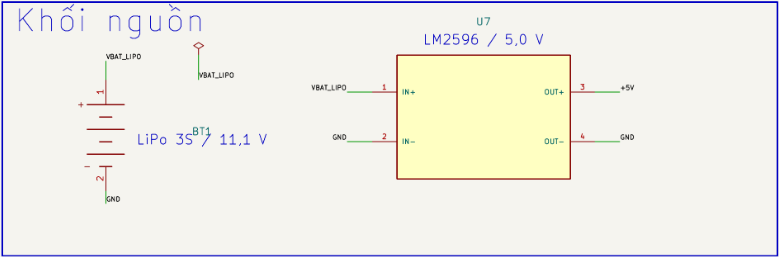
\includegraphics[trim=150bp 25bp 175bp 55bp,clip,width=0.55\linewidth]{figures/ch03/power-block.png}
	\caption{Sơ đồ nguyên lý khối nguồn.}
	\label{fig:design-power-block-schematic}
\end{figure}

Pin LiPo 3S cấp trực tiếp cho bốn ESC qua đường \texttt{VBAT\_LIPO}. Đường 5 V cấp cho bo STM32 và bộ thu ELRS được lấy từ mạch BEC tích hợp của ESC2; đầu ra BEC của ba ESC còn lại không kết nối. Tầng nguồn trên bo STM32 tạo đường 3,3 V cấp cho BMI160 và BNO055. Ba khối dùng chung GND làm mức điện áp tham chiếu cho nguồn và tín hiệu.

\clearpage
\subsection{Kết nối vi điều khiển với cảm biến và bộ thu}
\label{subsec:design-control-block}

\begin{figure}[H]
	\centering
	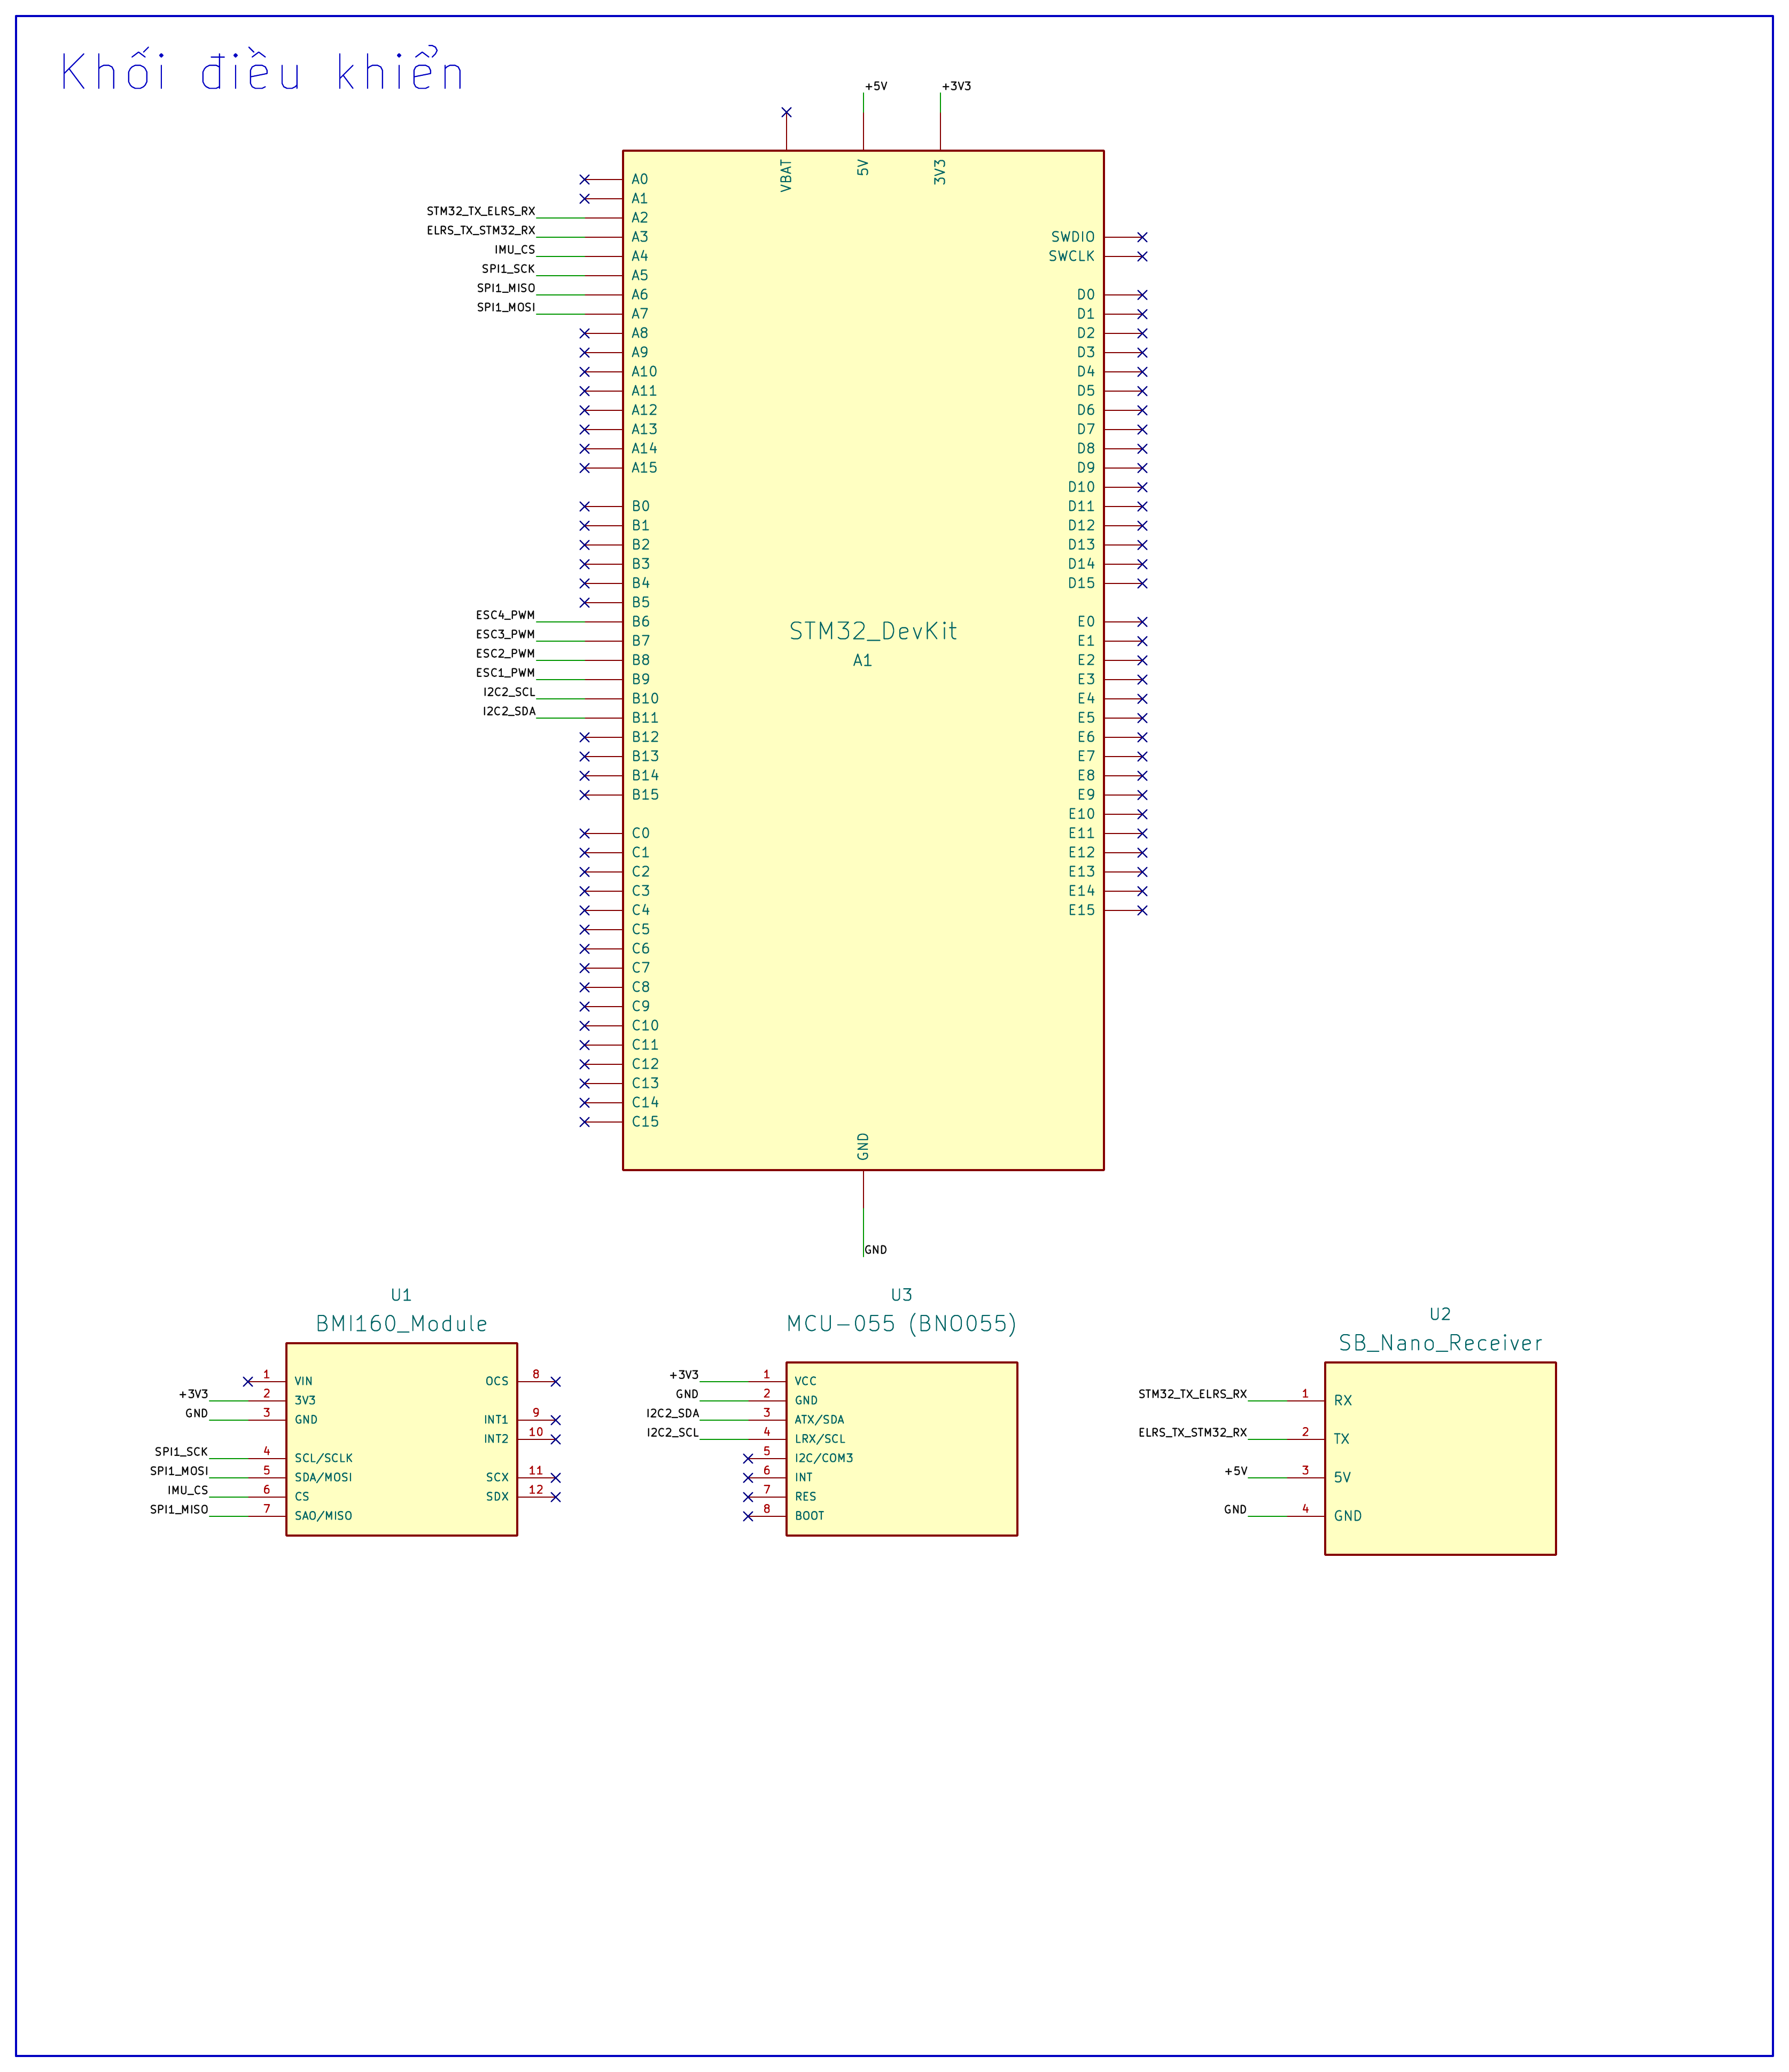
\includegraphics[trim=8bp 180bp 75bp 8bp,clip,width=\linewidth,height=16cm,keepaspectratio]{figures/ch03/control-block.png}
	\caption{Sơ đồ nguyên lý khối điều khiển.}
	\label{fig:design-control-block-schematic}
\end{figure}

Khối điều khiển gồm bo STM32F103VET6, BMI160, module BNO055 và bộ thu ELRS. BMI160 kết nối qua SPI1, sử dụng PA4 cho tín hiệu chọn chip, PA5 cho SCK, PA6 cho MISO và PA7 cho MOSI. BNO055 kết nối qua I\textsuperscript{2}C2 với PB10 là SCL và PB11 là SDA; hai cảm biến được cấp nguồn 3,3 V theo sơ đồ.

Bộ thu ELRS trao đổi dữ liệu với STM32 qua UART: PA2 nối tới RX của bộ thu, còn PA3 nhận dữ liệu từ TX của bộ thu. Các đường nguồn, GND và tín hiệu được liên kết giữa các module bằng nhãn mạng tương ứng trong sơ đồ.

\clearpage
\subsection{Kết nối ESC và động cơ}
\label{subsec:design-actuator-block}

\begin{figure}[H]
	\centering
	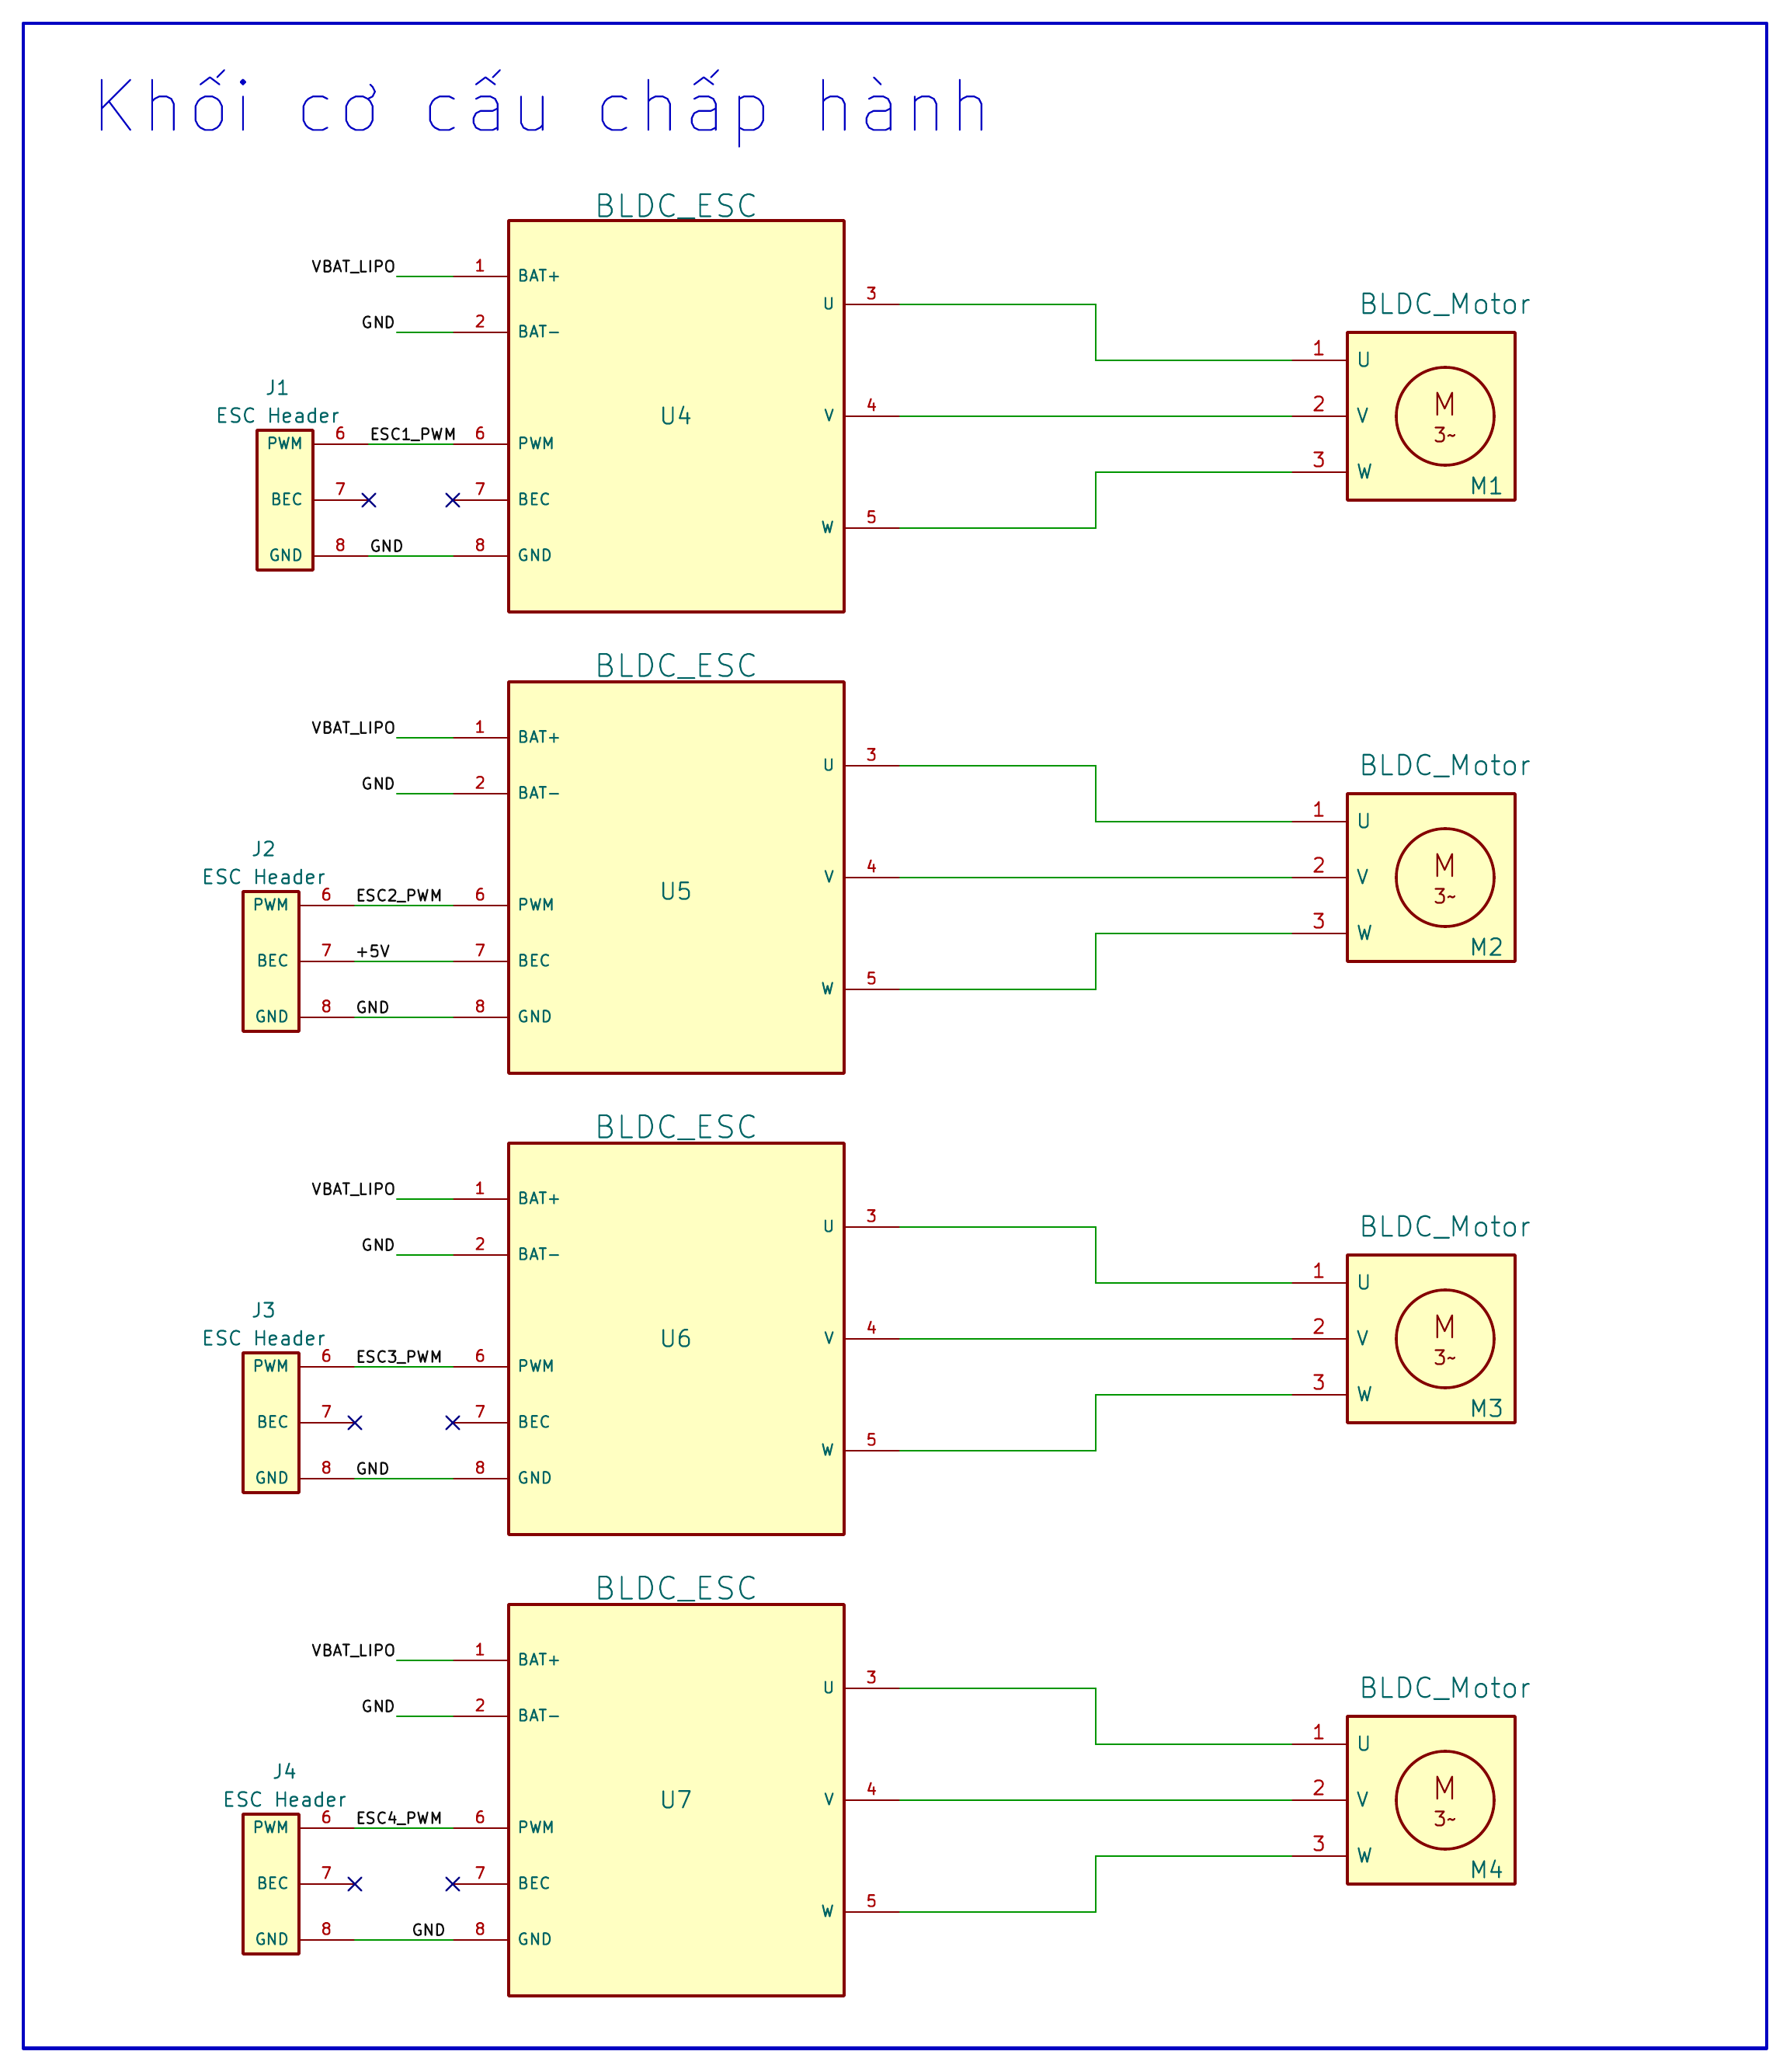
\includegraphics[trim=8bp 10bp 50bp 8bp,clip,width=\linewidth,height=17cm,keepaspectratio]{figures/ch03/actuator-block.png}
	\caption{Sơ đồ nguyên lý khối cơ cấu chấp hành.}
	\label{fig:design-actuator-block-schematic}
\end{figure}

Khối cơ cấu chấp hành gồm bốn tổ hợp ESC--động cơ--cánh quạt. Bốn lệnh PWM từ STM32 được đưa tới ESC1, ESC2, ESC3 và ESC4 lần lượt qua PB9, PB8, PB7 và PB6. Mỗi ESC nhận nguồn pin và lệnh PWM riêng, tạo ba pha U, V, W để điều khiển động cơ. Chênh lệch lực đẩy giữa bốn cụm tạo mômen hiệu chỉnh tư thế. Đường 5 V từ BEC của ESC2 được nối về khối điều khiển.
